\documentclass[12p]{article}

\usepackage{geometry} % Required to change the page size to A4
\geometry{a4paper} % Set the page size to be A4 as opposed to the default US Letter

\usepackage[utf8]{inputenc}
\usepackage{graphicx}
\usepackage{float} % Allows putting an [H] in \begin{figure} to specify the exact location of the figure
\usepackage{wrapfig} % Allows in-line images such as the example fish picture
\usepackage{lipsum} % Used for inserting dummy 'Lorem ipsum' text into the template
\usepackage{fancyhdr}
\usepackage[parfill]{parskip} % Makes sure to put line breaks in between paragraphs and have no indentation
\usepackage{dirtytalk} % Used for quotations (\say{quote}

\usepackage[
    style=numeric,
    sorting=none
    ]{biblatex}
\addbibresource{references.bib}

\linespread{1.2} % Line spacing

%\setlength\parindent{0pt} % Uncomment to remove all indentation from paragraphs

\graphicspath{{pics/}} % Specifies the directory where pictures are stored

%\pagestyle{fancy} %Don't use this

%----------------------------------------------------------------------------------------

\begin{document}

\newcommand{\HRule}{\rule{\linewidth}{0.5mm}} % Defines a new command for horizontal lines
\newcommand{\SlimHRule}{\rule{\linewidth}{0.25mm}} % Defines a new command for horizontal lines

%----------------------------------------------------------------------------------------
%	TITLE PAGE
%----------------------------------------------------------------------------------------

\begin{titlepage}
    
    \center
    
    %------------------------------------------------
	%	Logo
	%------------------------------------------------
	
	
\includegraphics[width=0.2\textwidth]{pics/AAU_Logo.png}\\[1cm]
    
    %------------------------------------------------
	%	Headings
	%------------------------------------------------
	
	\textsc{\LARGE Aalborg University Copenhagen}\\[1.5cm]
	
	\textsc{\Large P0 Project}\\[0.5cm]
	
	\textsc{\large Group 9}\\[0.5cm]
	
	\textsc{\large IT, Communication and New Media}\\[0.5cm]
	
	
	%------------------------------------------------
	%	Title
	%------------------------------------------------
	
	\HRule\\[0.4cm]
	
	{\huge\bfseries Quick Party}\\[0.4cm]
	
	\HRule\\[1.5cm]
	
	%------------------------------------------------
	%	Author(s) and Supervisor(s)
	%------------------------------------------------
	
	\begin{minipage}{0.4\textwidth}
    \begin{flushleft} \large
    \emph{Authors}\\
        Hamza \textsc{Al'akhir} \\
        Patryk \textsc{Gabryszak} \\
    	Gustav \textsc{Jørgensen} \\
    	Marius \textsc{Lungu} \\
    	Johannes \textsc{Mols} \\
    	Ruslan \textsc{Negrei} \\
    	Botis \textsc{Rares} \\
    \end{flushleft}
    \end{minipage}
    ~
    \begin{minipage}{0.4\textwidth}
    \begin{flushright} \large
    \emph{Study Numbers} \\
        - \\
        - \\
        20173797 \\
        20174691 \\
        20174921 \\
        - \\
        - \\
    \end{flushright}
    \end{minipage}\\[0.5cm]
    
    %------------------------------------------------
    
    \begin{minipage}{0.4\textwidth}
    \begin{flushleft} \large
    \emph{Supervisor}\\
        Lene Tolstrup \textsc{Sørensen} \\
    \end{flushleft}
    \end{minipage}
    ~
    \begin{minipage}{0.4\textwidth}
    \begin{flushright} \large
    \end{flushright}
    \end{minipage}\\[0.5cm]

	%------------------------------------------------
	%	Date
	%------------------------------------------------
	
	\vfill\vfill\vfill % Position the date 3/4 down the remaining page
	
	{\large\today} % Date, change the \today to a set date if you want to be precise
	
    
\end{titlepage}

%----------------------------------------------------------------------------------------
%	SYNOPSIS
%----------------------------------------------------------------------------------------

\begin{abstract}
    This project report describes the methods and processes of researching and developing an e-commerce shop. We chose to create an e-shop for alcohol delivery within Copenhagen to avoid the problem of closed shops during the night.
    \\ \\
    In order to realize this project, we used different common tools within marketing analysis, such as PEST and SWOT analysis, Blue Ocean - Red Ocean and stakeholder analysis. 
    \\ \\
    Using those research results, we created a technically functional e-shop with the popular content-management-system Wordpress.
\end{abstract}

\newpage

%----------------------------------------------------------------------------------------
%	TABLE OF CONTENTS
%----------------------------------------------------------------------------------------

\tableofcontents % Include a table of contents

\newpage % Begins the essay on a new page instead of on the same page as the table of contents 

%----------------------------------------------------------------------------------------
%	INTRODUCTION
%----------------------------------------------------------------------------------------

\section{Introduction}

\begin{center}
\vspace{1em}
\SlimHRule\\[0.1cm]
\Large{How can we make party supplies more accessible during night times, using the benefits of an easy-to-use ordering website and fast delivery service, and therefore provide an awesome party experience in the greater Copenhagen area?}
\SlimHRule\\[0.1cm]
\vspace{1em}
\end{center}

The above problem formulation focuses on a common problem among mostly younger people in today's society. During night times, most shops in Copenhagen are closed and bars are either too far away or too expensive, or both. Furthermore, most parties happen at private locations like apartments, where you can easily run out of supplies or you are simply too lazy to go to a shop and buy said supplies. This is where our service steps in. We provide a fast, reliable and secure service to deliver a broad variety of party supplies directly to the customer's doorstep. We make sure, the party never stops! 
\\ \\
Our product includes an easy ordering procedure through our website and a fast delivery by one of our employees. The supplies offered on our website are from a wide variety. We offer alcoholic beverages ranging from domestic and foreign beer to wine, vodka, whiskey and more, but also non-alcoholic beverages like coke (not the drug) and energy drinks. Furthermore, we are offering a great amount of party games like beer pong, card games, beer bongs and more. Alongside all of this, we also offer snacks and cigarettes. Special bundles for events like the \emph{Oktoberfest} are also included in our service.
\\ \\
Our target audience is mainly younger generations since they have the highest quantity of parties and also drink a lot more alcohol than older generations. We are hoping to especially appeal this audience with our variety of party games and special bundles. Nonetheless, anyone above the legal age is of course more than welcome to use our service.
\\ \\
The e-shop, which is described above, is only supposed to be an exemplary project, but not an actual business. We won't deliver products, nor take payments.

%----------------------------------------------------------------------------------------
%	EMPIRICAL DATA
%----------------------------------------------------------------------------------------

\newpage
\section{Empirical data}

%------------------------------------------------

\subsection{State of the art}

\subsubsection{Saucey \cite{Saucey}}
The website is for American citizens. It has a high-quality desktop interface including persuasive photos with drinking girls. It also has a high-quality logo, which defines their brand better.

Once you enter the main page, there is a button on "How it works" that sends you down the page, then it informs you that they have the best selection of wine, spirits and mixers. They also accentuate the fast delivery and the possibility of tracking your order with a simple click.

They feature some authoritative websites like the Los Angeles Times, Forbes and others. This is for building trust.

Further down the page, they display some testimonials of people who "love them", again, for making the customer to trust their service.

Furthermore, the website leads your journey through the website through positioning the "Get Started" button in the centre of the page along with a Zip Code or Address Field, making it easy for the customer to start his buying journey.

After you enter an address (for example, New York City) a grid-style based page appears with all the drinks available.

In this moment you can clearly see they intent to capture your attention in every possible manner, as you can find the top-right of each drink photo if a promotion is available.

Just below the main bar of the website, they display a search bar which searches for the input you type in (for example "wine" or "absolute vodka").

The overall appearance of the website, including the photos and the words used are quite persuasive, making sure, their service is the fastest possible, and they also try to appeal to the teenager customer by using words like "ASAP" or other slang used mainly by 18-25-year-old people.

The way they try to differentiate from the average alcohol delivery service is by offering a "book a bartender" option, if you really want to organize a big party.

\subsubsection{alkoXpress \cite{alkoXpress}}
This website is for Danish citizens in the northerly region of Zealand and they got a desktop interface which is easy to use. The design of the website is pretty simple as well. The usage of pictures and effects are minimized. At the top of the website, they have different kinds of “bars” which let you choose what drink you want. For example, the first bar is “Pakker” or “Package”. This will send you to a new page, where you can see all the different packages. 
\\ \\
Beyond alcohol, you can also buy cigarettes and accessories. The accessories are chips, cups and shot glasses etc. The order system is basic and easy to use, and if you have any kind of coupons to the website you can get some percentages off the price. 
Every drink is described when you click on them, for example, the Verdi Pomegranate 
“Gentle - sparkling - seductive - Italian.
Fresh with a comfortable well-balanced sweetness and a clean and light taste of pomegranate.
A beautiful sparkling tin based on natural ingredients.
Verdi Sparkletini is gluten-free”.
\\ \\
The package system is the way they try to differentiate from other alcohol delivery websites in Denmark. The audience of this website is younger people because of the names they use on the packages, such like “The King” “The Mexican” and “Beer pong”. 
\subsubsection{Allo Apéro Night \cite{alloAperoNight}}
The website offers service for french people located in Paris and greater Paris.
It’s purpose is very simple, delivering alcohol and drinks from 8pm to 6am.
The layout of the website is really simple and clean. They display a catalogue, which is very interactive, directly on the main page. They offer different kinds of alcohol, but also salads, accessories and soft drinks. 
\\ \\
The website has a dark themed vibe, that gives the users a sensation of premium services.
On the other hand, the lower part of the website is not well designed it and needs further polishing.
Their products are displayed in different categories such as beer, vodka, champagne, vine and so on.
When you click on one of them, you can see which brands they offer and there is a little description of the product.
The buying process is very generic. It’s the usual e-basket system, where you add your goods to the basket and then you have two options: either continue shopping or buy the goods.
\\ \\

You can also apply promotion codes.
The logo is very  simple, they have a catch phrase, which is that they deliver in 30 minutes maximum and their main emblem is the Eiffel tower.
Their consumer base is pretty large, ranging from 18 to 50 years of age, since shops close very early in Paris and there is no 24h super market.

%------------------------------------------------

\subsection{Literature review}

%----------------------------------------------------------------------------------------
%	MARKET ANALYSIS
%----------------------------------------------------------------------------------------

\newpage
\section{Market analysis} \label{MarketAnalysis}

%------------------------------------------------

\subsection{Methodology} \label{Methodology}

\newpage

%------------------------------------------------

\subsection{Analysis of external factors (PEST)} \label{PEST}

The purpose of a PEST analysis is to determine the external factors, which may have influence on the business, in both a positive and negative way. With such a report at hand, a business can make vital decisions in it's business plans to adapt to these factors in the best possible way. Since this business is based and operating in Copenhagen only, this analysis solely focuses on the Danish factors in politics, economy and society, while the technological factors are on a global scale.

\textbf{Political factors}

Since this business is mainly retailing alcohol, which is illegal to sell to minors, we have to oblige to certain laws in the danish legislation. There is no minimum age for consuming alcohol in Denmark, but there are multiple for selling it. The legal age for buying alcohol with a percentage below 16,5\% is 16, while it is 18 for everything above. The legal age to buy any alcohol in restaurants, bars, discos, etc. is 18. Tobacco and cigarettes are only sold to people above the age of 18 \cite{PEST_AlcoholAndTobaccoLegalAge}. It is also necessary to have a license from the municipal authorities, which is usually valid for eight years \cite{PEST_DenmarkAlcoholLaws}. Although selling "light" alcohol to persons above the age of 16 is legal, we will simply set the limit for our shop to 18, because we also offer hard alcohol and cigarettes and it is too complicated to separate the cases. The obvious conclusion out of these political factors is, that our e-shop needs a verification system to make sure, that every customer is of legal age. If we can not provide this, we are subject to fines and the license will most likely be taken away from our business. There are several ways of conducting an age verification. The easiest way to implement this, is probably by using existing systems like the CPR number or nemID, if that is possible. \\

\textbf{Economic factors}

With a nominal gross domestic product per capita of 52,87 thousand US dollars, Denmark is ranked as the 10th richest country in the world \cite{PEST_NominalGDPPerCapita}. It's economy experiences a modest growth each year, with 1,3\% in 2016 \cite{PEST_CIAFactbookDenmark}. Furthermore, Denmark is one of the oldest members of the European Union and is highly dependent on the free market and foreign trade in general. It has an opt-out agreement of the Euro, more specifically the ERM II agreement (European Exchange Rate Mechanism) \cite{PEST_ERM2}. In a nutshell, this agreement binds the exchange rate of the Danish Krone to never fluctuate more than $\pm$2,25\% to the Euro, which makes it a stable currency. The overall wealth, especially in Copenhagen, provides a stable market to create a business. The prices of our products will probably be rather high, because of the generally high prices of alcohol in Denmark, the high labour cost of the delivery service and the interest rate, which we have to take in order to stay in business and make profit. Finding workers will unlikely be an issue, since the work as delivery personnel does not require any level of education or skills and many students in Copenhagen are searching for small jobs besides their studies. Given the high amount of students in Copenhagen, our service has a large group of potential customers and therefore a good chance at dominating the market. \\

\textbf{Socio-Cultural factors}

It is well known, how important the danish drinking culture is. According to the official website of Denmark, beer has been a part of Danish culture for more than 5000 years. Every Dane drank around 80 litres of beer in 2010, and there are more than 100 breweries as of today \cite{PEST_BeerInDenmark}. Denmark has a very liberal opinion on alcohol and we won't have any problems with getting our business accepted within the society. In fact, the Danish culture gives us a lot of benefits to start a successful business by selling alcohol. \emph{Skål!} \\

\textbf{Technological factors}

As for the technological factors, it is relatively easy to set up an e-shop nowadays. With the technology of content-management-systems, you can set up a shop within minutes. The two hardest factors are: implementing an effective age verification system; and advertising the website to attract enough users.

\newpage

%------------------------------------------------

\subsection{Stakeholder analysis} \label{StakeholderAnalysis}

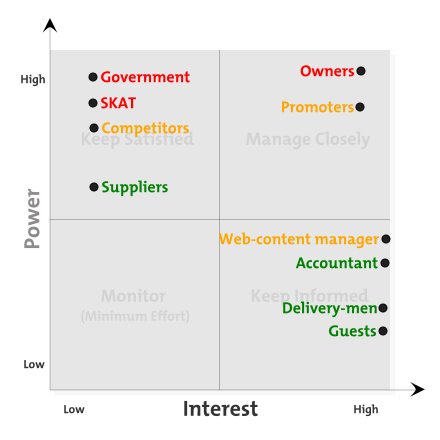
\includegraphics[width=1\textwidth]{stakeholder}\\
As seen in the diagram, we have prioritized our stakeholders in our project by influence and interest. In order to get most successful way to maintain a perfect work atmosphere, we need to provide every specific stakeholder with specific information. For each stakeholder we made the following information: 

\textbf{SKAT:}
In order to have our project/e-shop successful, we need to avoid problems with SKAT, because they have the influence to shut us down. The solution to fulfill their interest and prevent SKAT to shut us down we need to always use an account that always will make a track for our income and taxes, and also, the account should use an SKAT-consultant if the person has some questions.

\textbf{Government:}
Government has a high influence on our shop, as being an Alcohol selling e-shop, that could cause some problems if we get their non-wanted attention to us. Some of these things could be expired alcohol license, over-selling alcohol, selling alcohol to minors etc. Of course, we will follow all the laws and additional rules, but just in case, we will have put an extra effort while making deliveries or accounting the money.

\textbf{Competitors:}
Competitors are very important to every company, because the more you know competitors, we get better in an enrolled and unofficial competition with each other and also a better stability in the industry.

\textbf{Suppliers:}
Suppliers are the key value in our project, because if we have problems with them, we will have no products to sell in our e-shop. Therefore, we need to have a perfect relationship with them. The best way to get that is to follow the rules engaged by them and/or contract made between us. Also, follow an extra attention to thing as: Payment deadline, Missing information, Ignoring their warning, etc.

\textbf{Owners:}
Owners should have the closest managing attitude, because the consequences could lead to the termination of the project. In order to fulfill owners desired, the tasks and directions made by them should be followed by the employees, should be advised by promoters and web-content manager, and avoid errors at work by accountant and delivery-men.

\textbf{Promoters:}
Promoters have a very important role in our project, because if we don't promote our e-shop, there will be no sales, therefore no customers and no money. To help promoters do their job good, we need to provide them with no pressure, resources, information and other necessary things that they require.

\textbf{Web-content manager:}
Web-content manager is the face of our e-shop, as all the content, all the products are edited/made by him, and afterwards sold to the customers. We should provide him with required resources as: full information on products, full information on the company(that is shown to the customers on the website), all the new strategies of promoting(therefore he can change the packages/products on the website).

\textbf{Accountant:}
Accountant is the person that keeps the track of all the income, money used for resources, money used for law-purposes(such as consultants, licenses etc.), taxes. The most important thing that will keep her satisfied is that everybody makes all the money go through her, and of course, that will avoid any law problems in the future.

\textbf{Delivery-men:}
Delivery-men will be the people deliver our stuff to the customers, therefore if he fails to deliver different orders, we either will have a lot of complaints to our e-shop, or we will have no customers at all. To avoid this, we need to provide specific training's, resources(electric-mopeds, warm-suits for winter etc.), and a decent salary wage.

\newpage

%------------------------------------------------

\subsection{Market segmentation} \label{MarketSegmentation}

\textbf{What is market segmentation?}

Market segmentation is a term which refers to breaking down the total number of customers in groups based on common needs and similar responses to marketing approaches. This tactic is usually used by companies with the purpose of adhering to certain target groups (ex. teenagers) by making their product more appealing to that group.

\textbf{Why is it necessary?}

What makes this tactic necessary is the efficiency it provides. Instead of viewing all customers the same way, companies started spreading them in subgroups and creating new services or products destined to each of the categories they wanted to sell their product to, thus making the experience of every customer feel more personal and making them more likely to use the same product again. This has been observed by Emilly Hudell, the senior vice president of client sales and service at Turnkey Intelligence, who said market segmentation delivers more sales \cite{MarketSegmentationEfficieny}.

\textbf{How is it done?}

Market segmentation can be done by firstly learning what kind of consumers your product is more likely to attract and using this information to create a main category which you are going to sell to. By picking alcohol as our main product we expect our sales to be high since we are based in a city where alcohol is part of the culture and is used daily thus the demand is always present. From experience we have concluded that teenagers will be our main customers so we have made our shop as appealing as it could be to them by adding to our wares drinking games special packs, party organizing and cleaning services. By keeping a minimalist design, our site is easy to surf by people of all ages thus seeming more attractive for older people besides from the wide variety of high quality and low quality spirits which makes them available for every wallet.

\textbf{The main bases of market segmentation}

The main bases of market segmentation are geographic, demographic, behavioural and psycho-graphic. 

Geographically we chose to sell for the moment only in the city of Copenhagen as it is a densely populated region and there is a whole culture around consuming alcohol. This tradition can be used as means of boosting sales by having sales on important dates and events.

Demographically our goal is to have price ranges for every socio-economic group and any age or gender since locally everyone drinks more or less.

We are seeking to have our stocks available at all times so we can be seen as a reliable source of goods. Occasional price drops, offers, special packs, gift cards for loyal customers will make our shop more attractive to potential buyers.

\begin{figure}
    \centering
    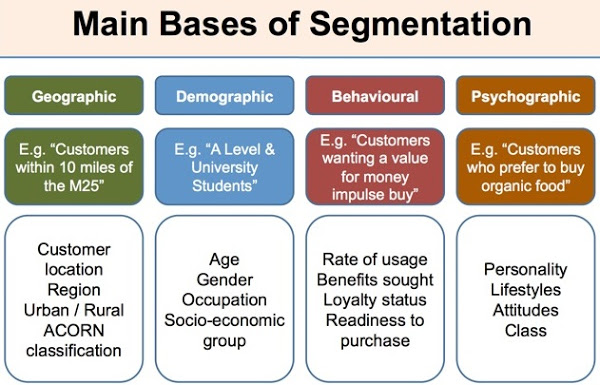
\includegraphics[width=1\textwidth]{market_segmentation}
    \caption{Main Bases of Segmentation \cite{MarketSegmentationBases}}
\end{figure}

\newpage

%------------------------------------------------

\subsection{Blue ocean - Red ocean} \label{BlueOceanRedOcean}

The Blue vs Red Ocean is a marketing theory which separates business in two different camps. The "Red" ocean is represented by a defined market filled with competitors ready to defeat their rivals either by lowering the price or delivering a better experience.

On the other side, in the "Blue" market there is little to no competition whatsoever, companies laying emphasis on development and research in order to discover these new markets and turn regular people into customers.

Even though this whole concept is manageable to understand by reading, we know for a fact that the actual positioning and how we can leverage certain aspects in order to widen the company angle instead of just picking a blue or a red side makes the actual difference between success and failure.

Although our company is already fixed by the market in the red ocean, we have thought about several ways on how can we use distinct marketing strategies to portray ourselves in front of customers as a "blue" ocean company instead of just being obliged to play by the "red" ocean rules, where the firm with the most resources usually wins.

We should also keep in mind that even though "to portray" may seem a little bit shallow, this is how big brands have established themselves as power players, by blending the actual service they were offering(a stale one) with some higher notes and colours, represented by slogans, branding or marketing, in all its forms and shapes. 

For this reason, instead of just targeting people who want to buy alcohol , we decided to add extra layers of targeting, narrowing our market to teens who live in Copenhagen Rural Areas, want to party and play the games they have already seen in the Hollywood blockbusters, without carrying any bag at all. Everything will be delivered right at their place, no matter the order time or the quantity needed.

Furthermore, a social media presence is vital in targeting our target market. Most likely tools like Instagram or Snapchat should be our primary focus, mostly because these platforms are more visual than Facebook, for example. However, we will use Facebook too, using the Paid advertisements to raise the awareness of the company and establish our brand as something unique, as we previously stated. 

%------------------------------------------------

\subsection{SWOT analysis} \label{SWOT}

\begin{table}[htbp]
  \centering
    \begin{tabular}{|p{0.5\textwidth}|p{0.5\textwidth}|}
    \hline
    \multicolumn{1}{|c|}{\textbf{Strengths}} & \multicolumn{1}{c|}{\textbf{Weaknesses}} \\
    \hline
    {• We can respond very quickly to our customers in Copenhagen and it's areas when they order on our platform\newline{}• Our prices are low and competitive compared to the market\newline{}• We know what our target customer is looking for if he chooses us, and therefore we can answer his needs very rapidly\newline{}• Our products are of certified good quality} & • Our company has little market presence or reputation\newline{}• We have a small staff, with limited skill base in many areas\newline{}• Higher price point compared to supermarkets since the service is included\newline{}• Delivery fees are higher by night time \\
    \hline
    \end{tabular}
  \label{tab:swot_one}
\end{table}

\begin{table}[htbp]
  \centering
    \begin{tabular}{|p{0.5\textwidth}|p{0.5\textwidth}|}
    \hline
    \multicolumn{1}{|c|}{\textbf{Opportunities}} & \multicolumn{1}{c|}{\textbf{Threats}} \\
    \hline
    {• Our competitors offer is very limited, so we can expand more over time\newline{}• The sector of alcohol is always growing, which leaves a gap in the market\newline{}• No real competitors in Denmark} & • Selling alcohol license may be hard to obtain\newline{}• Emergence of future competitors\newline{}• Customer choosing other options such as DøgnNetto, or Bilka \\
    \hline
    \end{tabular}
  \label{tab:swot_two}
\end{table}


\newpage

%------------------------------------------------

\subsection{The four P's}

This section will help us deliver a better product by analysing the market options in Copenhagen. By analysing the market, we can figure out what different kinds of products we want to distribute at a certain price. We will also find out which kind of promotion we want to use and what place we would be able to get the best opportunities. 

\begin{figure}[h]
    \center
    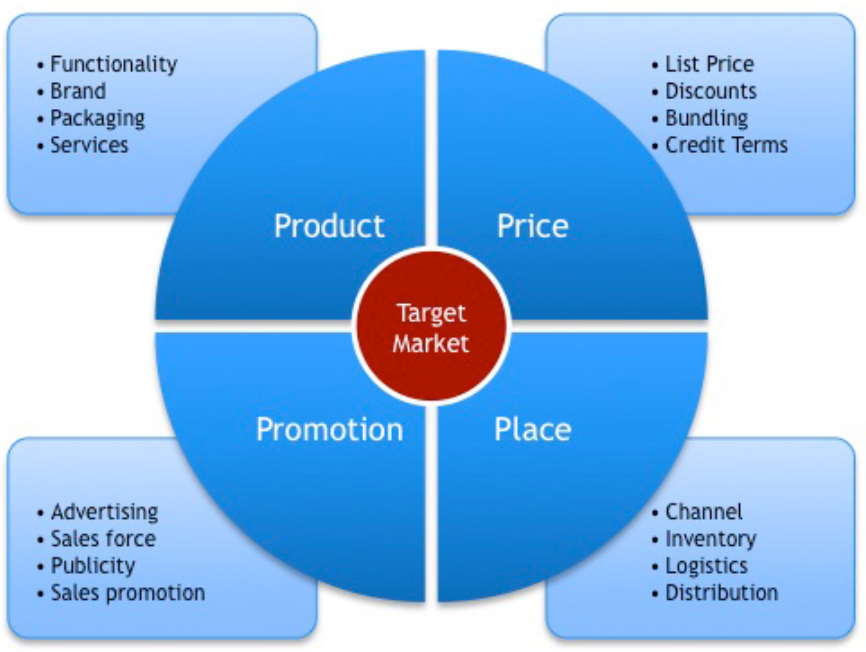
\includegraphics[width=0.6\textwidth]{4p}\\
\end{figure}

\label{PPPP}

\textbf{Product}

The products we have chosen are primarily alcohol and drinking games. We have chosen this product because of the drinking culture in Copenhagen. People in Copenhagen, both the youth and the elderly people often drink. The different categories of alcohol make our website more competitive against other websites selling alcohol because we have so many different variants of alcohol. We have all the big brands of alcohol, for example, we have \emph{Carlsberg}, \emph{Absolut Vodka}, \emph{Jack Daniels} and so on. Because of our big brand's people get more comfortable with buying alcohol from us, since we have recognized companies among our inventory. 
\\ \\
We have different kinds of packaging, which gets you a discount or maybe new entertainment to your current or future party. The packaging services include a game and some alcohol which create a drinking game. An example of a drinking game could be “Beer pong” which is very popular among the younger people playing drinking games. \\


\textbf{Price}

The price of our products will be cheap. But we still need to make some profit so our company can finance itself. We will have discounts so all of our products can attract new customers. Discounts and bundling of our products can help us sell more, and therefore gain a better and bigger capital for new products. New products and new prices are always good in our business since it can attract more customers. You can pay by credit card on our customer-friendly website. Find your products, and within a minute you have already paid for your alcohol to your current or future party.  \\

\textbf{Promotion}

The way we are going to promote our self, are primarily going to be on the social media, like Facebook, LinkedIn, Twitter and so on. We are trying to make way to our biggest customer. The youth. The youth are very active on the social media and we will try to find them there, by making funny or attractive ads. We also want to show us self in the public, by handing out flyers on the universities. \\


\textbf{Place}

We have chosen greater Copenhagen as our main goal. This is because of the huge amount of younger people and universities. We do not only target younger people here, but they are a huge factor in our selling prospects.
The drinking culture is very interesting here and people are drinking more than other cities. Most of the supermarkets sell alcohol until 23.00 every day, but after that most of the shops are beginning to close. Those who are not are only placed in the more central Copenhagen, which makes it difficult for people living in greater Copenhagen. 
\\ \\
We will distribute by car or bicycle depending on the distance. Our delivery will be efficient and fast. The ability to buy swiftly from our website makes your party even better when you are close to running out of alcohol. Our inventory will be stacked most of the time and we will ensure that our main products are available 24/7.

\newpage

%------------------------------------------------

\subsection{Marketing strategy} \label{MarketingStrategy}
Our Market strategy will be divided in two parts digital marketing and Sponsoring and events, the digital marketing section is a vital par for all start-ups nowadays.
So, we need a planning before launching our website and app to tease our services to customers.

Our first tool will be Facebook ads to track our potential clients Facebook and other Social Medias such as Snapchat and Instagram have surpassed TV ads today and attract more people so our strategy as a company is to take advantage of that, since our budget is limited and TV ads are expensive. 
For example, concluding sponsor-ships with well-known Danish Bloggers would be more efficient for us than using the normal TV ads methods since we will reach more our target customer.

Another good strategy would be search engine optimization, this means using smart tools such as good keywords, this will be the first step since we have no income in the beginning.
The second strategy will be SEM which will come at second stage this means our website will be better listed on the Google search engine therefore we will have a better exposure.

These two options will expand tremendously our client reach.
The last growing way of marketing would be YouTube videos/ads since YouTube is the most used website on the planet.
Many marketing strategies are possible for example YouTube Ads or creating our own YouTube Channel.

Sponsoring and events will be our second main Strategy marketing tool
For example, when it comes to YouTube we will be able to focus on partnering with YouTube Vloggers that likes the nightlife or having good times with friends.

We can also partnership with Local alcohol brands such as Carlsberg for example which would give us a great exposure.
Partnering with events companies or Festivals in Copenhagen is also a good marketing strategy this will also promotes our services and reach our target market.

When it comes to our first sponsors, university organizations such as IDA would be our best solution when we start our advertising campaign.
The target market is ideal since students like to play hard and party and since they are limited in time and money our service will provide them with all what they need. And to end this section we won’t make flyers because our target market does not pay attention to these kinds of advertisement.

\newpage

%----------------------------------------------------------------------------------------
%	WEBSITE DOCUMENTATION
%----------------------------------------------------------------------------------------

\newpage
\section{Documentation}

\subsection{WordPress}

\subsection{Setup}

\subsection{Products}

\subsection{Prices}

\subsection{Images}

%----------------------------------------------------------------------------------------
%	CONCLUSION
%----------------------------------------------------------------------------------------

\newpage
\section{Conclusion}

%----------------------------------------------------------------------------------------
%	BIBLIOGRAPHY
%----------------------------------------------------------------------------------------

\newpage
\printbibliography[heading=bibintoc,title={References}]

%----------------------------------------------------------------------------------------

\end{document}